
\chapter{Introduction}

This report details the design and implementation of a distributed computing system to solve exact cover problems.
Donald Knuth's Dancing Links (DLX) algorithm \cite{knuth00dancing} is used to solve the exact cover problems.
Exact cover is a general type of problem which can be applied to a wide range of problems.
It can be used to solve problems like $n$-queens, polyomino tiling, Latin square puzzles, Sudoku, set packing and set partitioning.
For more detailed information about how exact cover can be applied to $n$-queens, see Section \ref{queens_trans}.
% Applied to: polyomino tiling, Latin square and Sudoku

Distributed computing with this algorithm is accomplished by exploiting the recursive nature of DLX to split the problem into smaller pieces.
The Generic Distributed Exact Cover Solver (DECS) then takes advantage of a distributed computing middleware called BOINC \cite{boinc} to handle the work distribution and result collection process.
The report explains in detail how the DLX algorithm works and some concrete types of problems it can be applied to.
It also looks at some of the important aspects of the implementation as well as some simulation and test results.
%It also explains how DLX is used together with BOINC to construct a complete distributed computing system.



\section{Queens}
\label{intro_queens}

The 8-queens problem asks how eight queens can be placed on an $8 \times 8$ chessboard so that no two queens attack each other.
In chess a queen can attack horizontally, vertically and diagonally on the board.
Figure \ref{fig:8queens-invalid} might appear to be a valid solution at first sight, but more careful study shows that the queens at B1 and H7 are attacking each other, thus rendering this configuration invalid.
Figure \ref{fig:8queens} shows a valid solution to the eight queens problem.
Depending on the symmetries in the solution up to seven other solutions can easily be found by rotating the board 90, 180 and 270 degrees.
By turning the board upside down and applying the same rotations the other four solutions can be found.
The 8-queens problem has a total of 92 configurations where none of the queens attack each other.

$n$-queens is the generalized form of the 8-queens problem where $n$ queens are placed on an $n \times n$ board.
A number of different algorithms exist to find all the solutions to a given $n$-queens problem.
This report will show the details of how the DLX algorithm is able to solve the $n$-queens problem.

\begin{figure}[hptb]
	\centering 
	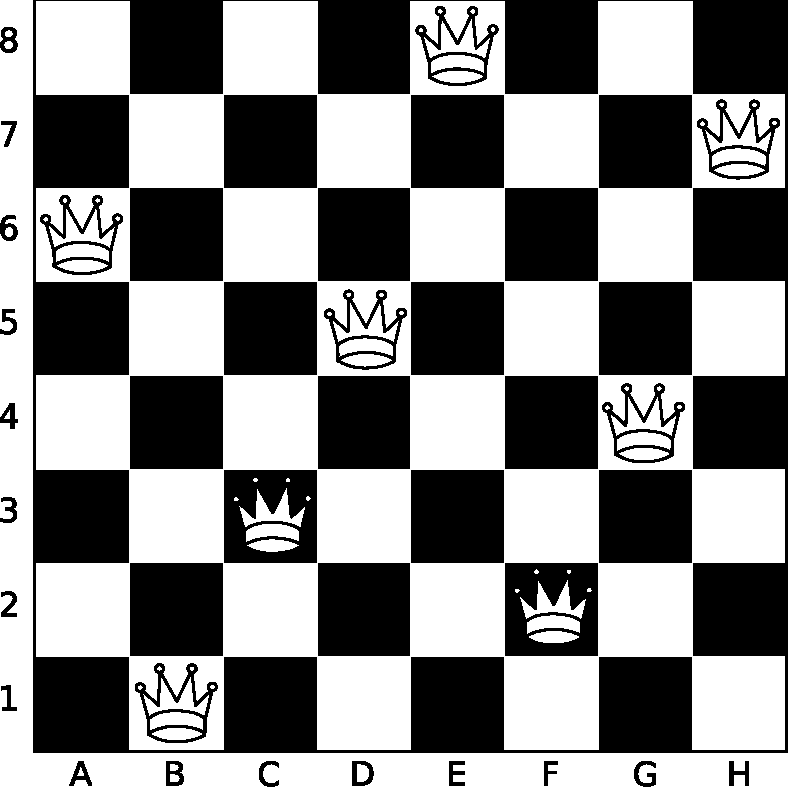
\includegraphics[width=0.65\textwidth]{queens-invalid.pdf}
	\caption{Board configuration where the queens at B1 and H7 attack each other}
	\label{fig:8queens-invalid}
\end{figure}

\begin{figure}[hptb]
	\centering 
	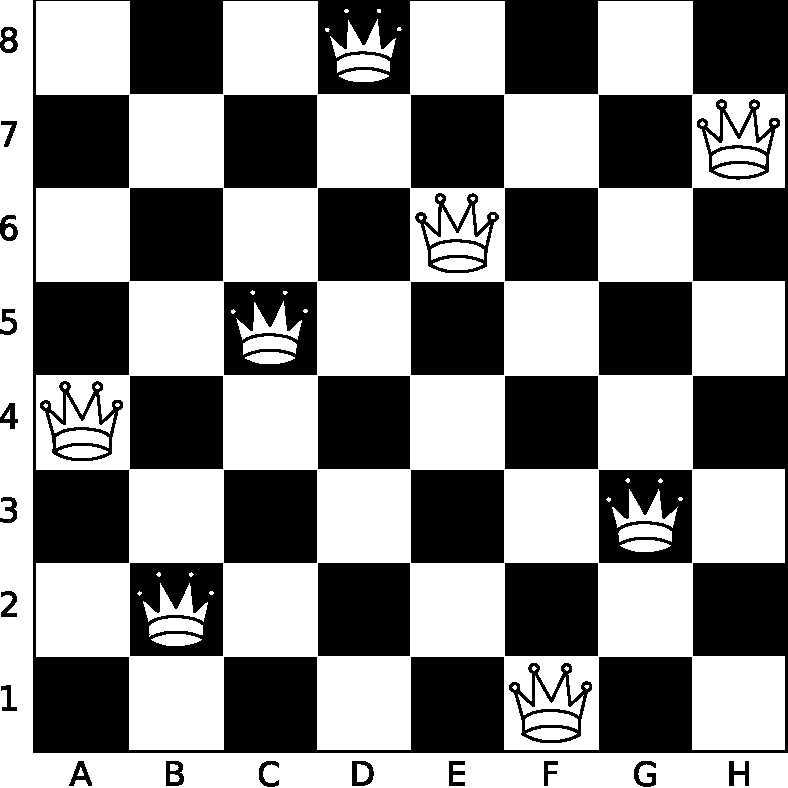
\includegraphics[width=0.65\textwidth]{queens-basic.pdf}
	\caption{One possible solution to the 8-queens problem}
	\label{fig:8queens}
\end{figure}



\section{Related work}

There are numerous implementations of the Dancing Links algorithm available with and without source code.
In addition to Knuth's own implementation in CWEB \cite{cweb} a quick search found source code for Java, Python, C, C++, Ruby, Lisp, Haskell, MATLAB and Mathematica.
Some of the implementations were generic while others aimed for a specific application (mostly Sudoku).
Common for all these implementations is that none of them were designed for parallel processing.

Alfred Wassermann developed a parallel version of Knuth's algorithm in \cite{wassermann99covering} by using PVM \cite{pvm} to solve a problem presented in Knuth's original paper.
Matthew Wolff also developed a parallel version and with the help of MPI \cite{QuinnMPI} he used it to find solutions to the $n+k$ queens problem \cite{ChathamQueens}.
However, Wassermann and Wolff only published the solutions to their respective problems and not the actual implementations they used.
The only available open source parallel version is written by Owen O'Malley for the Apache Hadoop project \cite{hadoop} in May 2007.
O'Malley's implementation uses the MapReduce framework \cite{map-reduce} provided by Hadoop to do the computations in parallel.
The details of this implementation and how it divides the problem into smaller pieces has, to the author's knowledge, not been published.



\section{Report organization}

This report is organized into several chapters.
Chapter \ref{dancing_links} describes the Dancing Links algorithm.
Chapter \ref{implementation} discusses different aspects of the implementation.
Chapter \ref{testing} describes the some simulation and test results and Chapter \ref{conclusion} concludes this report.
